% The five write-ups in one PDF, in dependency order. Each chapter keeps its own numbering,
% which matches its Markdown version and the Lean references in the code.
% Build with ../build.sh (no arguments), after the chapter PDFs exist.
\documentclass[11pt]{article}
\usepackage[margin=1in]{geometry}
\usepackage{pdfpages}
\usepackage[hidelinks,bookmarksnumbered]{hyperref}

\title{Convergence Rates of Actor-Critic Methods\\[2pt]\large Notes with Lean formalization}
\author{Vijaymohan Konda}
\date{\today}

\begin{document}
\pagenumbering{roman}
\maketitle
\thispagestyle{empty}

\noindent These notes collect five write-ups. Each chapter is a self-contained document with its
own numbering of theorems and equations, as in its Markdown version in \texttt{docs/}. Each
formalized statement is followed by a \emph{Lean} note naming its theorem in \texttt{RLTheory/},
and the last section of Chapter~5 lists what is checked in Lean. To check a statement, build the
library (\texttt{lake build}) and run \texttt{\#print axioms} on the named theorem. The expected
output is \texttt{[propext, Classical.choice, Quot.sound]}.

\medskip\noindent Dependencies: Chapter~5 uses the policy gradient $\nabla J$ of Chapter~1 and the
covariance theorems of Chapters~3 and~4. The trace-driven noise of Chapter~3 uses the closed-form
covariance of Chapter~2.

\tableofcontents
\clearpage
\pagenumbering{arabic}

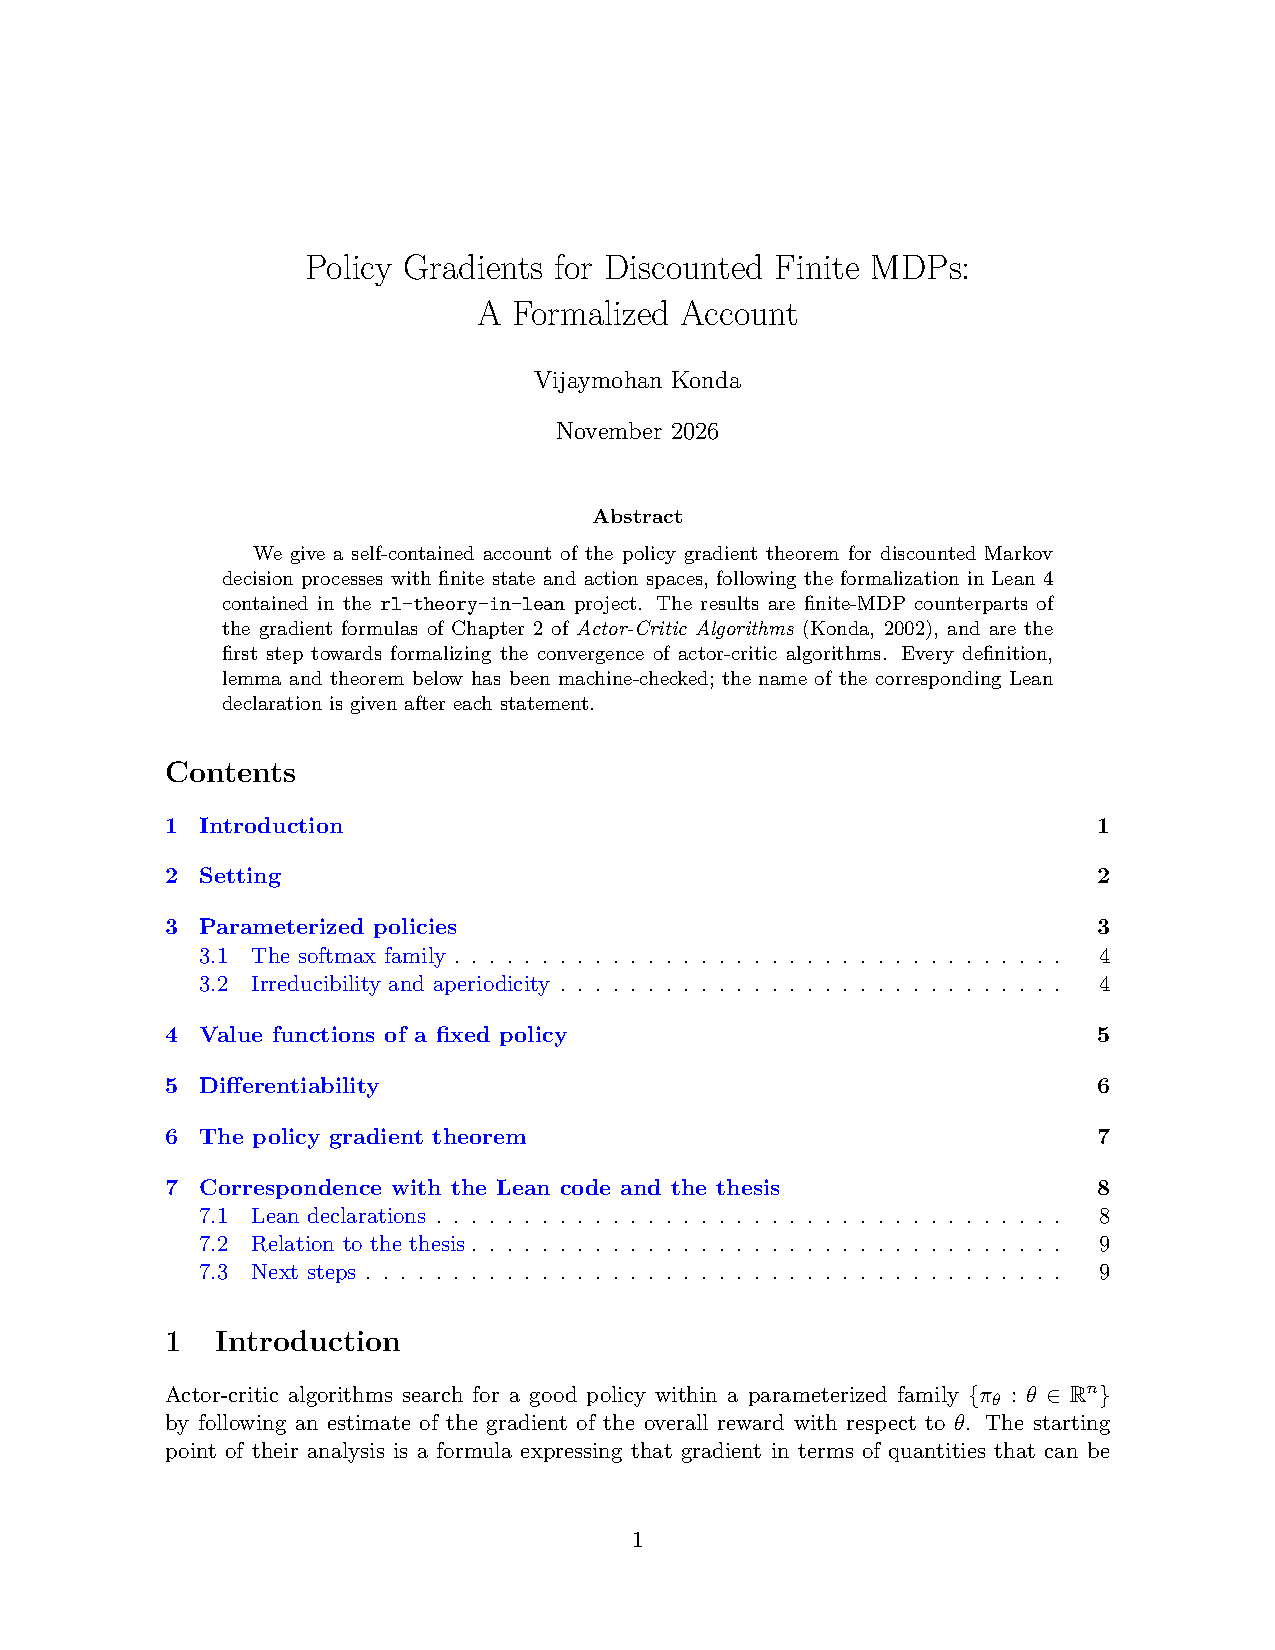
\includepdf[pages=-,pagecommand={\thispagestyle{empty}},
  addtotoc={1,section,1,{Policy gradients for discounted finite MDPs},ch:pg}]{../policy-gradient.pdf}
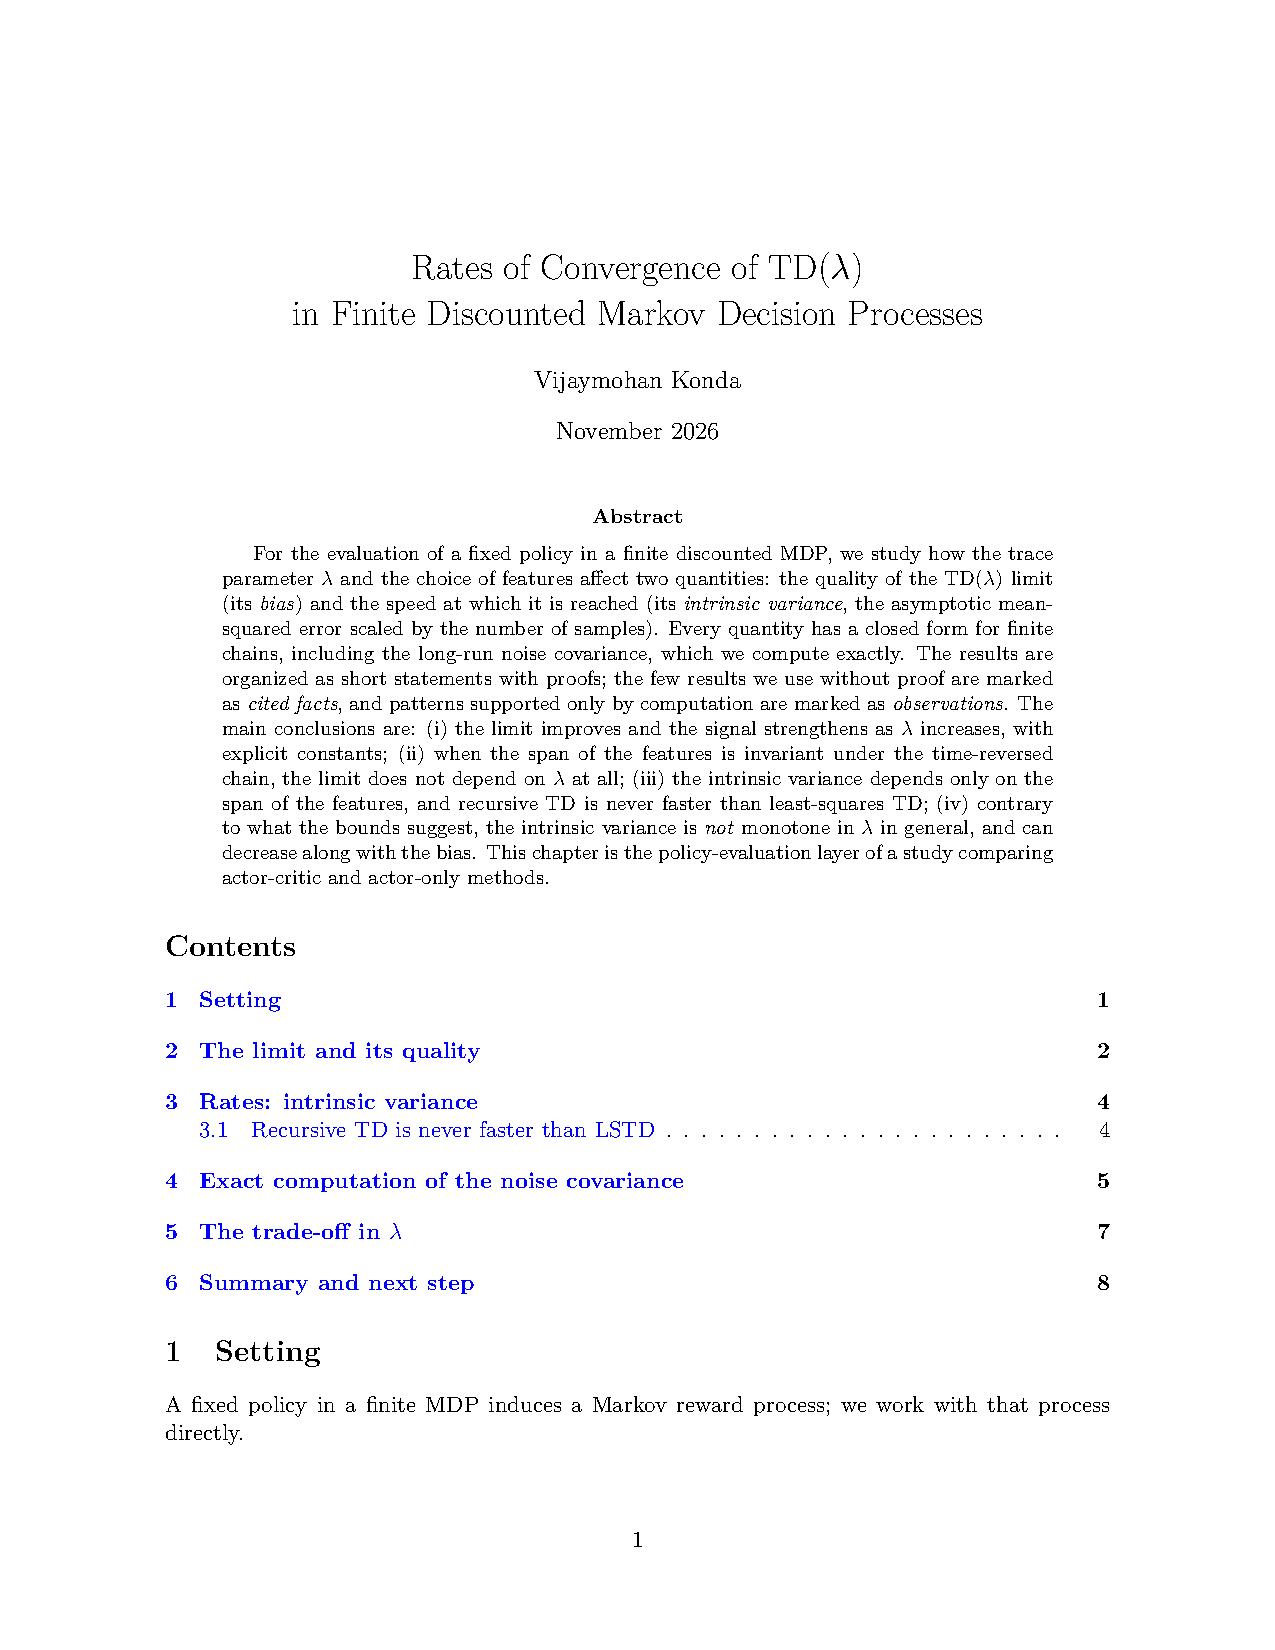
\includepdf[pages=-,pagecommand={\thispagestyle{empty}},
  addtotoc={1,section,1,{Rates of convergence of TD($\lambda$)},ch:td}]{../td-lambda-rates.pdf}
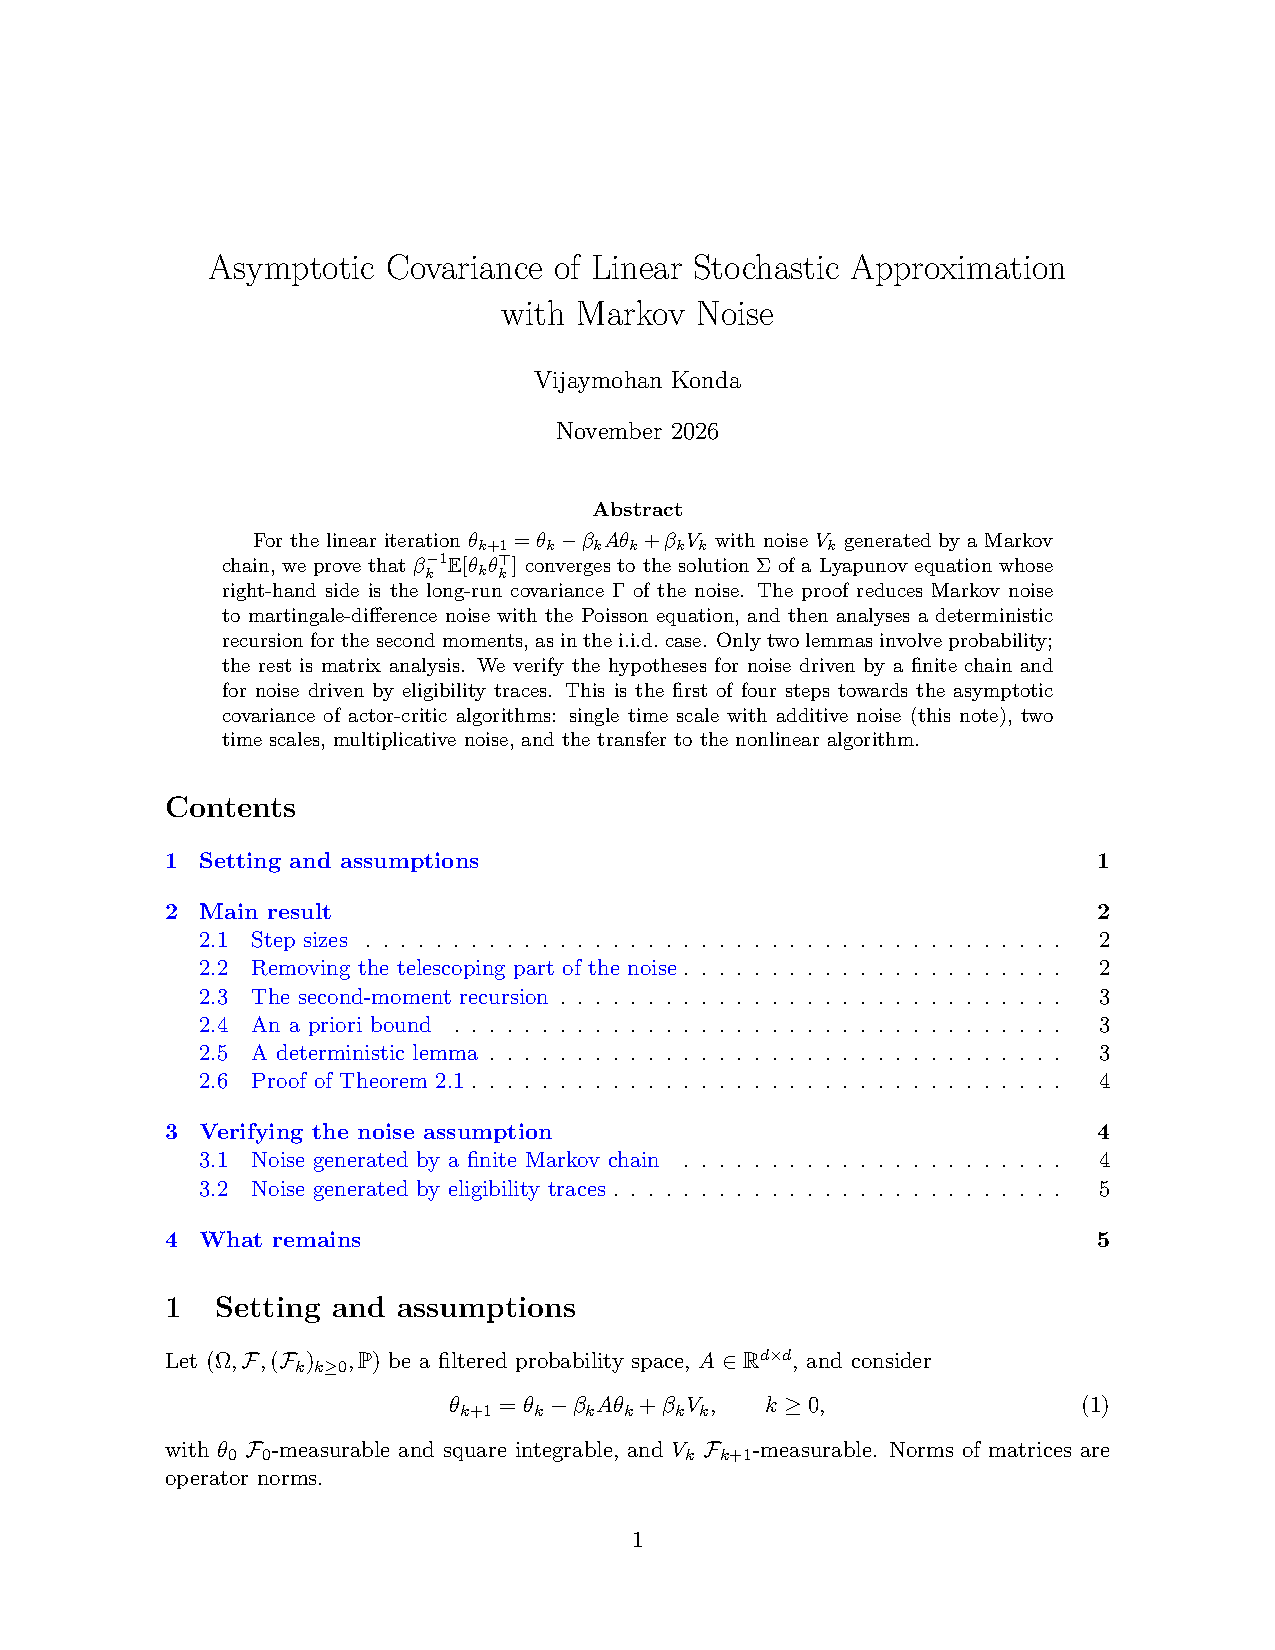
\includepdf[pages=-,pagecommand={\thispagestyle{empty}},
  addtotoc={1,section,1,{Asymptotic covariance of linear SA with Markov noise},ch:cov}]{../markov-sa-covariance.pdf}
\includepdf[pages=-,pagecommand={\thispagestyle{empty}},
  addtotoc={1,section,1,{Two-time-scale SA with Markov noise},ch:tts}]{../two-time-scale-covariance.pdf}
\includepdf[pages=-,pagecommand={\thispagestyle{empty}},
  addtotoc={1,section,1,{Rates of actor-critic and actor-only methods},ch:ac}]{../actor-critic-rates.pdf}

\end{document}
